\documentclass[12pt]{article}

\usepackage{amsmath, mathtools}
\usepackage{amsfonts}
\usepackage{amssymb}
\usepackage{graphicx}
\usepackage{colortbl}
\usepackage{xr}
\usepackage{hyperref}
\usepackage{longtable}
\usepackage{xfrac}
\usepackage{tabularx}
\usepackage{float}
\usepackage{siunitx}
\usepackage{booktabs}
\usepackage{caption}
\usepackage{pdflscape}
\usepackage{afterpage}
\usepackage{enumitem}
\usepackage[round]{natbib}

%\usepackage{refcheck}

\hypersetup{
   % bookmarks=true,         % show bookmarks bar?
      colorlinks=true,       % false: boxed links; true: colored links
    linkcolor=red,          % color of internal links (change box color with linkbordercolor)
    citecolor=green,        % color of links to bibliography
    filecolor=magenta,      % color of file links
    urlcolor=cyan           % color of external links
}

%% Comments

\usepackage{color}

\newif\ifcomments\commentstrue

\ifcomments
\newcommand{\authornote}[3]{\textcolor{#1}{[#3 ---#2]}}
\newcommand{\todo}[1]{\textcolor{red}{[TODO: #1]}}
\else
\newcommand{\authornote}[3]{}
\newcommand{\todo}[1]{}
\fi

\newcommand{\wss}[1]{\authornote{blue}{SS}{#1}}
\newcommand{\an}[1]{\authornote{magenta}{Author}{#1}}



% For easy change of table widths
\newcommand{\colZwidth}{1.0\textwidth}
\newcommand{\colAwidth}{0.13\textwidth}
\newcommand{\colBwidth}{0.82\textwidth}
\newcommand{\colCwidth}{0.1\textwidth}
\newcommand{\colDwidth}{0.05\textwidth}
\newcommand{\colEwidth}{0.8\textwidth}
\newcommand{\colFwidth}{0.17\textwidth}
\newcommand{\colGwidth}{0.5\textwidth}
\newcommand{\colHwidth}{0.28\textwidth}

% Used so that cross-references have a meaningful prefix
\newcounter{defnum} %Definition Number
\newcommand{\dthedefnum}{GD\thedefnum}
\newcommand{\dref}[1]{GD\ref{#1}}
\newcounter{datadefnum} %Datadefinition Number
\newcommand{\ddthedatadefnum}{DD\thedatadefnum}
\newcommand{\ddref}[1]{DD\ref{#1}}
\newcounter{theorynum} %Theory Number
\newcommand{\tthetheorynum}{T\thetheorynum}
\newcommand{\tref}[1]{T\ref{#1}}
\newcounter{tablenum} %Table Number
\newcommand{\tbthetablenum}{T\thetablenum}
\newcommand{\tbref}[1]{TB\ref{#1}}
\newcounter{assumpnum} %Assumption Number
\newcommand{\atheassumpnum}{P\theassumpnum}
\newcommand{\aref}[1]{A\ref{#1}}
\newcounter{goalnum} %Goal Number
\newcommand{\gthegoalnum}{P\thegoalnum}
\newcommand{\gsref}[1]{GS\ref{#1}}
\newcounter{instnum} %Instance Number
\newcommand{\itheinstnum}{IM\theinstnum}
\newcommand{\iref}[1]{IM\ref{#1}}
\newcounter{reqnum} %Requirement Number
\newcommand{\rthereqnum}{P\thereqnum}
\newcommand{\rref}[1]{R\ref{#1}}
\newcounter{lcnum} %Likely change number
\newcommand{\lthelcnum}{LC\thelcnum}
\newcommand{\lcref}[1]{LC\ref{#1}}

\newcommand{\progname}{ProgName} % PUT YOUR PROGRAM NAME HERE

\usepackage{fullpage}

\begin{document}

\title{CAS 741: SRS \\A Numerical Search For The Spectrum Related To Travelling 
Periodic Waves} 
\author{Robert White}
\date{\today}
	
\maketitle

~\newpage

\pagenumbering{roman}

\section{Revision History}

\begin{tabularx}{\textwidth}{p{3cm}p{2cm}X}
\toprule {\bf Date} & {\bf Version} & {\bf Notes}\\
\midrule
25-09-2018 & 1.0 & Creation of the first draft\\
29-09-2018 & 1.1 & Edit of 1.0. Added a GS, responsibilites, requirenments, 
definitions and verification of compatibility. Updated comments.tex. My 
comments are in red, SS comments are in blue.\\ 
01-10-2018 & 1.2 & Edit of 1.1. Added more theory to support the instance 
model. Made a clearer distinction between user and reader charaterisitcs. 
Modified the goal statements.  \\ 
03-10-2018 & 1.3 & Edit of 1.2. Removed a redundant goal statement. Made some 
of Dr. 
Smith's suggested changes. Updated the traceability matrices.  \\
04-10-2018 & 1.4 & Edit of 1.3. Created IM2 and inserted tracebility graphs. 
Completed all of Dr. Smith's suggested changes. Performed a grammar and 
spelling check.\\ 
11-10-2018 & 1.5& Edit of 1.4. Draft 1.4 was peer reviewed by Hanane Zlitni. 
Most of her recommended changes were made. \\
\bottomrule
\end{tabularx}

~\newpage

\section{Reference Material}

This section records information for easy reference.

\subsection{Table of Units}

Throughout this document SI (Syst\`{e}me International d'Unit\'{e}s) is employed
as the unit system.  In addition to the basic units, several derived units are
used as described below.  For each unit, the symbol is given followed by a
description of the unit and the SI name. \\

~\newline

\renewcommand{\arraystretch}{1.2}
%\begin{table}[ht]
  \noindent \begin{tabular}{l l l} 
    \toprule		
    \textbf{symbol} & \textbf{unit} & \textbf{SI}\\
    \midrule 
    \si{\metre} & length & metre\\
    t & time & second\\
    \bottomrule
  \end{tabular}
  %	\caption{Provide a caption}
%\end{table}


\subsection{Table of Symbols}

The table that follows summarizes the symbols used in this document along with
their units. Some of the symbols are unitless, 
they are marked with a dash. The choice of symbols was made to be consistent 
with the rogue 
wave and mathematical physics literature.  

\renewcommand{\arraystretch}{1.2}
%\noindent \begin{tabularx}{1.0\textwidth}{l l X}
\noindent \begin{longtable*}{l l p{12cm}} \toprule
\textbf{symbol} & \textbf{unit} & \textbf{description}\\
\midrule 
$\lambda$ & $\frac{1}{s}$ & spectral parameter
\\
$u$ & m & wave amplitude 
\\  
$\phi$ & - & eigen function
\\ 
$c$ & $\frac{m}{s}$ & wave speed 
\\
$\omega$ & $\frac{1}{s}$ & angular frequency 
\\ 
$e$ & - & euler's Number \\ 
$i$ & - & imaginary number\\ 
$(g,d)$ & - & conserved quantities\\
  
\bottomrule
\end{longtable*}

\subsection{Abbreviations and Acronyms}

\renewcommand{\arraystretch}{1.2}
\begin{tabular}{l l} 
  \toprule		
  \textbf{symbol} & \textbf{description}\\
  \midrule 
  A & Assumption\\
  $\mathbb{C}$ & Complex numbers\\
  cn & Elliptic cosine \\
  DD & Data Definition\\
  dn & Delta amplitude \\ 
  GD & General Definition\\
  GS & Goal Statement\\
  IM & Instance Model\\
  LC & Likely Change\\
  NLS & Nonlinear Schrodinger\\
  ODE & Ordinary Differential Equation\\
  PDE & Partial Differential Equation\\
  PS & Physical System Description\\
  $\mathbb{R}$ & Real number line\\
  R & Requirement\\ 
  sn & Elliptic sine\\
  SRS & Software Requirements Specification\\
  \progname{} & SpecSearch\\
  T & Theoretical Model\\  
  \bottomrule
\end{tabular}\\

\subsection{Mathematical Notation}

Let $\delta$ be a complex number of the form $\delta= m + ni$ ($m,n \in 
\mathbb{R}$). The real part of u is m and the imaginary part of u is n. $i$ is 
the imaginary number such that $i=\sqrt{-1}$.\\

The complex 
conjugate of $\delta$ is defined to be $\bar{\delta}= m - ni$. 
The modulus of $u$ is defined to be $|\delta| = \sqrt{m^{2}+n^{2}}$.\\

Let $z(x,t): \mathbb{R}^{2} \rightarrow \mathbb{C}$. We will let $z_{t}$ and 
$z_{x}$ denote 
the partial derivatives of $z$ with respect to t and x respectively. If $z$ has 
one independent 
variable we will denote its derivative by $z'$. \\ 

$ z_{t} = \lim_{h \to 0 } \frac{z(x,t+ t_{0}h) - z(x,t)}{h}$ \\ 

Where $z_{t}$ is differentiable if the above limit is the same regardless of 
the complex number (direction) $t_{0}$. \\

If H is a matrix then $H_{t}$ 
is the 
matrix formed by taking the t derivative in each component of $H$.\\ 

$ e^{i \omega t} = cos(\omega t) + i sin(\omega t)$. So it is clear from the 
above definitions that \\

$ |e^{i \omega t}| = \sqrt{sin^{2} (\omega t) + cos^{2} (\omega t)} =1$ \\  

To see this consider the angle $\omega t$ for fixed $t$. Let the opposite side 
be $a$, denote 
the adjacent side by $b$ and the hypotenuse by $c$. This forms a right angle 
triangle (see picture below). By definition,  $sin(\omega t) = \frac{a}{c} $ 
and $ cos(\omega t) = \frac{b}{c} $. Now, by pythagoras we have that\\

$ \sqrt{sin^{2} (\omega t) + cos^{2} (\omega t)} = 
\sqrt{\frac{a^{2}+b^{2}}{c^{2}} } = \sqrt{ \frac{c^{2}}{c^{2} } }= 1 $ \\ 

For each t. So $e^{i \omega t}$ stays on the complex unit circle. \\

\begin{figure}[h!]
	\begin{center}
		{
			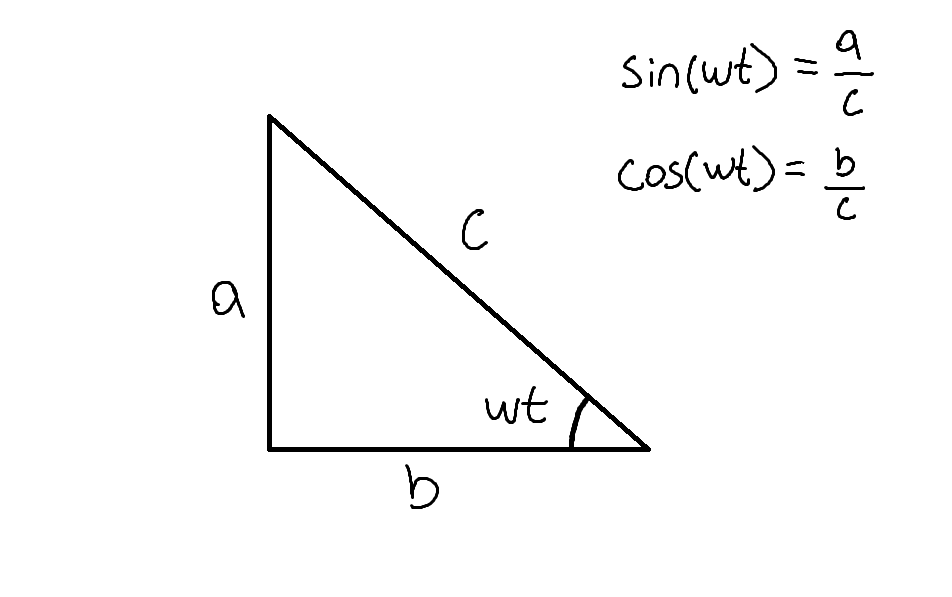
\includegraphics[width=\textwidth]{pytha.png}
		} 
	\caption{Trigonometric Ratios}
	\end{center}
\end{figure}

\newpage
\tableofcontents



\pagenumbering{arabic}
\newpage 
\section{Introduction}

\subsection{Purpose of Document}
The purpose of this document is to describe the requirements for the spectral 
search program (SpecSearch). SpecSearch will search for the 
continuous spectrum of a lax pair that is compatible with solutions 
of the NLS 
equation. \\ 

This document will explain the mathematical models, assumptions, 
solution characterisitcs and goals of the software. After reading this document 
one should be able to understand the mathematical and physical context of the 
inputs and outputs. They should also recognize the connections and 
dependencies between these SRS topics. \\

The SRS is meant to be simaltaneously unambigious and abstract. It details the 
quality attributes of the software, such as functionality, 
without dicussing any code, numerical algorithms or scientific computing 
solutions. It is a precursor to the documents required in the development of 
scientific software. One should read and understand this document before the 
VnV, design or code itself. 

\subsection{Scope of Requirements} 

The scope of SpecSearch is limited to finding the spectrum of a particular 
linear lax equation and determining the stability of the corresponding waves. 
The waves being investigated are solutions to 
the focusing NLS equation. 

\subsection{Characteristics of Intended Reader} 

The reader of this document should have taken an introductory course 
in partial differential equations and complex analysis. They should also have a 
first year undergraduate understanding of linear algebra.

\subsection{Organization of Document}

This document follows a template provided by Dr. Spencer Smith at McMaster 
University. It begins by introducing the document. This introduction is 
followed by a general overview of the system and then an outline of the goals 
and mathematical theory. The document continues by describing the behaviour 
between inputs 
and outputs, judging output and then foreshadows changes to the software. It 
concludes with useful graphs and figures for tracebility. \\ 

More details of the template can be found in Smith et al (2005) and Smith et al 
(2007). The latex template is available in Dr. Spencer Smith's gitlab 
repository CAS 741. 

\section{General System Description}

This section identifies the interfaces between the system and its environment,
describes the user characteristics and lists the system constraints.

\subsection{System Context} 
Diagram 1 shows the system context. The circle represents the user of the 
scientific software. The rectangle resembles the software system. The arrows 
indicate the flow of data between software and environment. 
 \begin{figure}[h!]
	\begin{center}
		{
			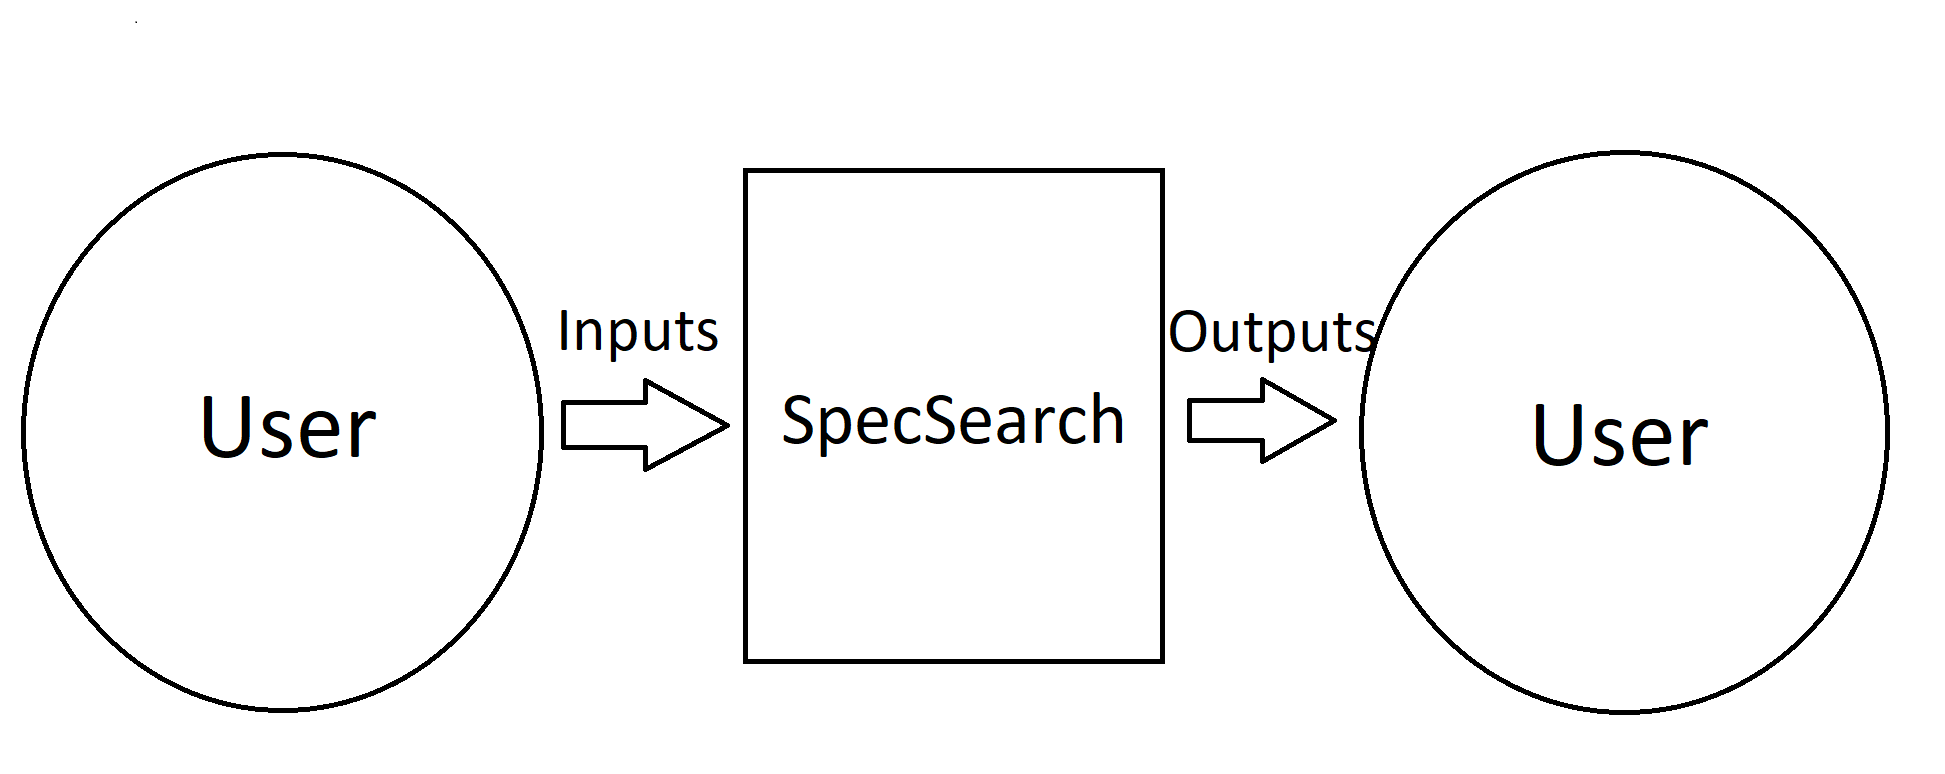
\includegraphics[width=15cm,height=6cm]{SystemContext.png}
		} 
	\caption{System Context}
	\end{center}
 \end{figure}

\begin{itemize}
\item User Responsibilities:
\begin{itemize}
\item Ensure that the input variables resemble the wave that you intend 
to analyze.
\item Ensure that the assumptions imposed on waves in this software are 
reasonable 
for your reasearch.
\item Ensure that the software is used in a legal and ethical manner.

\end{itemize}
\item SpecSearch Responsibilities:

\begin{itemize}
\item Detect data type mismatch. 
\item Solve the lax equation associated with the given wave parameters. 
\item Connect the discrete spectrum in order to form a continuous spectrum. 
\item Display the continuous spectrum on the complex plane.
\item Determine whether or not the waves are stable. 
\end{itemize}
\end{itemize}

\subsection{User Characteristics} \label{SecUserCharacteristics}

The user should have a basic understanding of wave mechanics (wave 
speed, 
amplitude and angular frequency). They should also understand the concept of 
conserved quantities. 

\subsection{System Constraints}

My supervisor requires that software will be created with MATLAB.


\section{Specific System Description}

This section first presents the problem description, which gives a high-level
view of the problem to be solved.  This is followed by the solution 
characteristics specification, which presents the assumptions, theories, 
definitions and finally the instance models. 

\subsection{Problem Description} \label{Sec_pd}
A lax pair is a set of matrices or operators that satisfy differential 
equations. The NLS equation, a PDE used to model rogue waves and modulated wave 
packets, appears as a compatibility condition of a particular lax pair of 
equations. One equation is a spectral problem, with matrix U, and the other is 
a time evolution problem, with matrix V. See instance model 1 for more 
details.\\

 The 
spectral problem is important because the spectral 
parameter within it contains information about the stability of solutions. See 
instance model 2 for more details regarding stability.\\

SpecSearch will attempt to produce a numerical approximation of the continuous 
spectrum for the previously mentioned spectral problem. In particular, 
it will find the spectrum for general travelling periodic wave solutions of the 
focusing
NLS equation. \\ 

Previous attempts have used an algebraic method to calculate the spectral 
parameter (Pelinovsky 2018)(Deconinck 2017). These attempts have only been 
successful at finding a countable number of points on the spectrum. This 
software will 
search for more points and "connect" the points in an attempt to approximate 
and search for the continuous spectrum.  

\subsubsection{Terminology and  Definitions}

This subsection provides a list of terms that are used in the subsequent
sections and their meaning, with the purpose of reducing ambiguity and making it
easier to correctly understand the requirements:

\begin{itemize}

\item \textbf{Spectrum}: The set of allowable values for the spectral parameter 
of a matrix or operator.
\item \textbf{Operator}: A mapping that transforms elements of a space into 
other elements of the same space. 
\item \textbf{Traveling Periodic Wave}: A periodic and one-dimensional wave 
that travels with a constant speed, c, and angular frequency, $\omega$. 
\item \textbf{Compatibility Condition}: Conditions for which the lax pair of 
equations is guaranteed. 
\item \textbf{Stability}: A solution is stable if slight perturbations in 
initial conditions lead 
to slight perturbations in the entire solution.
\item \textbf{Initial Data}: The graph of a wave (or its derivative) 
at a fixed point in time, tyically t=0.
\item \textbf{Rogue Wave}: A wave is considered rogue if its amplitude is more 
than double of the average of the upper third wave amplitudes in its 
surroundings. 
\item \textbf{PDE}: A partial differential equation.An equation containing one 
or more partial derivatives. The partial derivative of a multivariable function 
is a derivative with respect to one of its arguments. 
\item \textbf{Countable:} A set that is finite or has the same cardinality as 
the natural numbers (1,2,3,4,5 ....). 
\item \textbf{Focusing wave:} When the nonlinear Schr\"{o}dinger equation adds 
the 
nonlinear term ($+|u|^{2}u$).  
\item \textbf{Hamiltonian:} Is an operator corresponding to the total energy of 
a system. 

\end{itemize}

\subsubsection{Physical System Description}

The physical system of SpecSearch includes the following elements:

\begin{itemize}

\item[PS1:] 
Unspecified body of water or laser channel with a traveling periodic 
wave.

\end{itemize}

\subsubsection{Goal Statements}

\noindent Given the constant wave speed,c , angular frequency ,$\omega$, 
conserved quantities, (g,d), and the intial profile of a general traveling 
periodic wave, the goal statements are:

\begin{itemize}[leftmargin=.75in]

\item[GSlocate:] {Locate elements of the continuous spectrum on the 
complex plane. }

\item[GSstable:] {Determine the stability of the solutions.}

\end{itemize}

\subsection{Solution Characteristics Specification}

The instance model that governs SpecSearch is presented in
Subsection~\ref{sec_instance}.  The information to understand the meaning of the
instance models and their derivation is also presented, so that the instance
models can be verified.

\subsubsection{Assumptions}

This section simplifies the original problem and helps in developing the
theoretical model by filling in the missing information for the physical
system. The numbers given in the square brackets refer to the theoretical model
[T], general definition [GD], data definition [DD], instance model [IM], or
likely change [LC], in which the respective assumption is used.

\begin{itemize}[leftmargin=.5in]

\item[Aham:]The 
wave equation is a complex hamiltonian evolution equation. 
\item[Amom:]The 
linear momentum densities are proportional to the integrands of the 
corresponding velocity functionals 
\item[Awav:]All 
waves in the model are general traveling perioidic waves with constant speed 
and frequency. 
\item[Anls:]The 
wave is a solution to the NLS equation.
\item[Afoc:]The 
system only deals with focusing waves.
\item[Astat:] The system will start by assuming that the wave is stationary and 
then use 
the stationary solution to build the moving solution.

\end{itemize}

\subsubsection{Theoretical Models}\label{sec_theoretical}

This section focuses on the general equations and laws that SpecSearch is based
on. 
~\newline

\noindent
\begin{minipage}{\textwidth}
	\renewcommand*{\arraystretch}{1.5}
	\begin{tabular}{| p{\colAwidth} | p{\colBwidth}|}
		\hline
		\rowcolor[gray]{0.9}
		Number& T1\\
		\hline
		Label&\bf Focusing NLS for General travelling periodic waves\\
		\hline
		Equation&  $ u'' + 2|u|^{2}u+2icu'=\omega u$\\
		\hline
		Description & 
		General traveling periodic waves that satisfy the Schr\"{o}dinger 
		equation 
		will have this form. \\
		\hline
		Source &
		Deconinck (2017)\\
		% The above web link should be replaced with a proper citation to a 
		%publication
		\hline
		Ref.\ By & DD1, IM1\\
		\hline
	\end{tabular}
\end{minipage}\\ 

\begin{center}
\newpage
\begin{flushleft}
	\textbf{Derivatition of the Focusing NLS for 
		General Traveling Periodic 
		Waves}
\end{flushleft} 

\end{center} 

We start with the focusing NLS equation: $iq_{t} + q_{xx} + 
2|q|^{2}q=0$ \\ 

The NLS equation is a PDE meant to model modulated wave packets and rogue waves 
in physics. $u$ is the complex envelope of the wave, $t$ is time and $x$ is the 
position in one dimensional space. \\ 

A general traveling periodic wave has the form $z(x,t)=u(x+2ct)e^{i \omega 
t}$.$(u: \mathbb{R} \rightarrow \mathbb{C})$. 
We will now search for general traveling periodic waves that are solutions to 
the NLS equation. This is done by setting z=q in the NLS equation. This 
yields: \\ 
\begin{center}
$ iz_{t} + z_{xx} + 2|z|^{2}z = 0$ \\ 
$ \Rightarrow i(2cu'e^{i \omega t} + i \omega ue^{i \omega t}) + u''e^{i \omega 
t} + 2|u|^{2}|e^{i \omega t}|^{2} u e^{i \omega t} = 0 $ \\
 $\Rightarrow e^{i \omega t} (2icu' + i^{2} \omega u + u'' + 2|u|^{2}u) = 0 $ 
 \\ 
$ \Rightarrow 2icu' - \omega u + u'' + 2|u|^{2}u =0$ \\ 
\end{center}
Which is the result in T1.

\subsubsection{General Definitions}\label{sec_gendef}

There are no general definitions.

\subsubsection{Data Definitions}\label{sec_datadef}

This section collects and defines all the data needed to build the instance
models. 
~\newline

\noindent
\begin{minipage}{\textwidth}
\renewcommand*{\arraystretch}{1.5}
\begin{tabular}{| p{\colAwidth} | p{\colBwidth}|}
\hline
\rowcolor[gray]{0.9}
Number& DD\refstepcounter{datadefnum}\thedatadefnum \label{FluxCoil}\\
\hline
Label& \bf Conservation Equations\\
\hline
Symbols &$g, c, d, \omega$\\
\hline
% Units& $Mt^{-3}$\\
% \hline
  SI Units & -\\
  \hline
  Equation(1)&$\bar{u}u' - u\bar{u}' + 2ic|u|^{2} = 2ig$\\
  Equation(2)&$|u'|^{2} + |u|^{4} + d = \omega |u|^{2}$\\
  \hline
  Description & 
                These are conserved quantities in the NLS equation. For fixed 
                g and d the above relations are true for all space and time.
  \\
  \hline
  Sources& Deconinck (2017) \\
  \hline
  Ref.\ By & IM1\\
  \hline
\end{tabular}\\
\end{minipage} 

\begin{center}
	\newpage
	\begin{flushleft}
		\textbf{Justification of a Conserved Quantity}
	\end{flushleft} 
	
\end{center} 

I will first multiply T1 by $\bar{u}$. \\ 
\begin{center}
$  u''\bar{u} + 2|u|^{2}u \bar{u}+2icu' \bar{u}=\omega u \bar{u}$ (*) \\ 
\end{center}
Taking the complex conjugate yields: \\ 
\begin{center}
$ \bar{u''} u + 2|u|^{2} \bar{u} u -2ic\bar{u'}u = \omega \bar{u} u$ (**) \\ 
\end{center} 
Subtraction of * with ** yields: \\ 
\begin{center} 
$  u''\bar{u} + 2|u|^{2}u \bar{u}+2icu' \bar{u} - (\bar{u''} u + 2|u|^{2} 
\bar{u} u -2ic\bar{u'}u) =\omega u \bar{u} - (\omega \bar{u} u)$\\ 
$ \Rightarrow  u''\bar{u} - \bar{u''} u + 2ic (u' \bar{u} + \bar{u'}u ) = 0$ \\
$ \Rightarrow \int u''\bar{u} - \int \bar{u''} u + 2ic \int (u' \bar{u} + 
\bar{u'}u ) = 2ig  $ \\  
\end{center} 
Noticing that the term in the integral attatched to 2ic is a product rule.\\ 
\begin{center}
$ \Rightarrow \int u''\bar{u} - \int \bar{u''} u + 2icu \bar{u} = 2ig $ \\
$ \Rightarrow \bar{u}u' - \int \bar{u'} u' - u \bar{u'} + \int \bar{u'} u' + 
2icu \bar{u} = 2ig$ \\ 
$ \Rightarrow \bar{u}u' - u\bar{u}' + 2ic|u|^{2} = 2ig$ \\ 
\end{center} 
The second conserved quantity is obtained by multiplying $\bar{u'}$ by T1, 
adding the complex conjugate and integrating. 

\subsubsection{Instance Models} \label{sec_instance}    

This section transforms the problem defined in Section~\ref{Sec_pd} into 
one which is expressed in mathematical terms. It uses concrete symbols defined 
in Section~\ref{sec_datadef} to replace the abstract symbols in the models 
identified in Sections~\ref{sec_theoretical} and~\ref{sec_gendef}. \\

The goals GSlocate and GSstable are solved by IM1 and IM2 respectively.  

%Instance Model 1

\noindent
\begin{minipage}{\textwidth}
\renewcommand*{\arraystretch}{1.5}
\begin{tabular}{| p{\colAwidth} | p{\colBwidth}|}
  \hline
  \rowcolor[gray]{0.9}
  Number& IM\refstepcounter{instnum}\theinstnum \label{ewat}\\
  \hline
  Label& \bf Searching for the continuous spectrum\\
  \hline
  Input&$c, \omega, g, d$, initial wave profile\\
  \hline
  Output&$\lambda$ such that:\\
  &$\phi_x = U(u,\lambda) \phi$\\
  \hline
  Description& $U(u,\lambda) = \begin{pmatrix} 
  \lambda & u \\
  -\bar{u} &-\lambda 
  \end{pmatrix}$ \\
  &T1 is a compabililty condition for the lax pair comprised of the above row's 
  ODE and $\phi_{t}=V(u,\lambda)\phi$\\
  &$V(u,\lambda)=i \begin{pmatrix} 
  2 \lambda^{2} + |u|^{2} & u_{x}+2 \lambda u \\
  \bar{u}_{x}-2\lambda \bar{u} & -2\lambda^{2} - |u|^{2}
  \end{pmatrix}$ \\
  &$\phi \in \mathbb{C}$\\
  \hline
  Sources& Deconinck (2017) \\
  \hline
  Ref.\ By & IM2\\
  \hline
\end{tabular}
\end{minipage}\\
 

\begin{center}
	\begin{flushleft}
		\textbf{Justification of Compatibility Conditions}
	\end{flushleft} 
	
\end{center} 
For a smooth $C^{2}$ function ,$\phi$, we have that $\phi_{tx}=\phi_{xt}$. \\
From IM1 $\Rightarrow \phi_{xt} = \delta_{t} U \phi + UV \phi$ and $\phi_{tx} = 
\delta_{x} V \phi + VU \phi$. \\
Combining the above two equations : \\ 

$\Rightarrow \delta_{t} U \phi + UV \phi = \delta_{x} V \phi + VU \phi$ \\
$\Rightarrow \delta_{t} U + UV = \delta_{x} V + VU$ (--) \\ 
$\Rightarrow$
$\begin{pmatrix} 
	0 & u_{t} \\
	-\bar{u}_{t} & 0
\end{pmatrix}$ +
$i \begin{pmatrix} 
\lambda & u \\
-\bar{u} & -\lambda
\end{pmatrix}$ 
$ \begin{pmatrix} 
2\lambda^{2} + |u|^{2} & u_{x}+2\lambda u \\
\bar{u}_{x} -2\lambda\bar{u} & -2\lambda^{2} - |u|^{2}
\end{pmatrix} =$ 
$ i \begin{pmatrix} 
u_{x}\bar{u} + u\bar{u}_{x} & u_{xx} + 2\lambda u_{x} \\
\bar{u}_{xx} - 2 \lambda \bar{u}_{x} & -u_{x} \bar{u} - u_{x}\bar{u}_{x}
\end{pmatrix} +$ 
$i \begin{pmatrix} 
2 \lambda^{2} + 2|u|^{2} & u_{x} + 2\lambda u_{x} \\
\bar{u}_{x} - 2 \lambda \bar{u} & -2 \lambda^{2} - |u|^{2}
\end{pmatrix}$ 
$\begin{pmatrix} 
	\lambda & u \\
	- \bar{u} & - \lambda
\end{pmatrix}$
\\
$\Rightarrow \begin{pmatrix} 
	i(2 \lambda ^{3} + \lambda |u|^{2} + u\bar{u}_{x} -2\lambda |u|^{2}) & 
	u_{t} + i(\lambda u_{x} + 2 \lambda^{2} u - 2 \lambda^{2} u - u|u|^{2}) \\
	-\bar{u}_{t} + i(-2 \lambda^{2}\bar{u} - \bar{u}|u|^{2} - 
	\lambda\bar{u}_{x} + 2 \lambda^{2} \bar{u}) & i(-\bar{u} u_{x} - 2 \lambda 
	u \bar{u} + 2 \lambda^{3} + \lambda |u|^{2})
\end{pmatrix} $ = \\
$ i \begin{pmatrix} 
	u_{x}\bar{u} + u\bar{u}_{x} + 2 \lambda^{3} + \lambda |u|^{2} - 
	u_{x}\bar{u} - 2\lambda |u|^{2} & u_{xx} + 2\lambda u_{x} + 2\lambda^{2} u 
	+ u|u|^{2} - 2|u|^{2} - \lambda u_{x} \\
	\bar{u}_{xx} - 2\lambda \bar{u}_{x} + \lambda \bar{u}_{x} - 
	2\lambda^{2}\bar{u} + 2\lambda^{2}\bar{u} + \bar{u}|u|^{2} & -u_{x}\bar{u} 
	- u_{x}\bar{u}_{x} + u\bar{u}_{x} - 2\lambda |u|^{2} + 2\lambda^{3} + 
	\lambda |u|^{2}
\end{pmatrix}$ \\
$ \Rightarrow \begin{pmatrix} 
0 & u_{t} - iu|u|^{2} \\
-\bar{u}_{t} - i\bar{u}|u|^{2} & 0
\end{pmatrix} $ = 
$ \begin{pmatrix} 
0 & iu_{xx} + iu|u|^{2} \\
i\bar{u}_{xx} + i \bar{u}|u|^{2} & 0
\end{pmatrix} $ \\ 
% new line
$ \Rightarrow \begin{pmatrix} 
0 & iu_{t} + 2u|u|^{2} + u_{xx} \\
iu_{t} + 2u|u|^{2} + u_{xx} & 0
\end{pmatrix} $ = 
$ \begin{pmatrix} 
0 & 0 \\
0 & 0
\end{pmatrix} $ \\ 


This is true if u satisfies the NLS equation (T1). Thus, the NLS equation is a 
compatibility 
condition for the lax pair in IM1. \\

\noindent
\begin{minipage}{\textwidth}
	\renewcommand*{\arraystretch}{1.5}
	\begin{tabular}{| p{\colAwidth} | p{\colBwidth}|}
		\hline
		\rowcolor[gray]{0.9}
		Number& IM\refstepcounter{instnum}\theinstnum \label{ewat}\\
		\hline
		Label& \bf Stability\\
		\hline
		Input &$\lambda, \omega, g, d$\\
		\hline
		Output& Stable or Unstable \\ 
		\hline
		Description& $\Omega = \frac{+}{-} 2i (\lambda^{4} - \frac{1}{2}\omega 
		\lambda^{2} - ig\lambda + \frac{1}{16}\omega^{2} - 
		\frac{1}{4}d)^{\frac{1}{2}}$ \\
		& If the real part of $\Omega > 0$  then the solution, u, 
		is unstable. \\
		\hline
		Sources& Deconinck (2017) \\
		\hline
		Ref.\ By & IM2\\
		\hline
	\end{tabular}
\end{minipage} \\

\begin{center}
	\begin{flushleft}
		\textbf{Validation of Stability Criteria}
	\end{flushleft} 
	
\end{center} 

Without loss of generality it is possible to set $c=0$. \\  

We can write $\phi(x,t) = M(t) \chi (x,t) $. Here M(t) is the diagonal matrix 
with the first entry as $e^{\frac{i \omega t}{2}}$ and second entry as 
$e^{\frac{-i \omega t}{2}}$ and $\sigma_{3}$ is the diagonal matrix with top 
entry 1 and bottom entry -1.\\  

Substituting this into the lax pair in IM1 yields: \\ 
\begin{center} 
$\chi _{x} = U \chi $ and $\chi_{t} = V \chi - \frac{i \omega}{2} \sigma_{3} 
\chi$ \\ 
Let $\chi (x,t) = e^{t \Omega} \phi (x) $. \\ 
$\Rightarrow \Omega \phi = V(u,\lambda) \phi - \frac{i \omega}{2} \sigma_{3} 
\phi$ \\ 
\end{center} 
This matrix system admits a non zero solution when the determinant of the 
following:
\begin{center}  
$ R(\Omega, \lambda) = \begin{pmatrix} 
i(2\lambda^{2} + |u|^{2} - \frac{\omega}{2}) - \Omega & i(u_{x}+2\lambda u) \\
i(\bar{u}_{x}-2\lambda \bar{u}) & -i(2\lambda^{2} + |u|^{2} - \frac{\omega}{2}) 
- \Omega
\end{pmatrix} $ \\  
\end{center} 
Is nonzero. Expanding the determinant of R it follows that: \\ 
\begin{center}
$|R| = \Omega^{2} + 4(\lambda^{4} - \frac{1}{2} \omega \lambda^{2} + 
\frac{1}{16} \omega^{2} - \frac{1}{4}d ) = \Omega^{2} +4P(\lambda) = 0$ \\ 
$ \Rightarrow \Omega^{2} = -4P(\lambda)$ \\ 
$ \Rightarrow \Omega = \frac{+}{-}\sqrt{-4P(\lambda)} $\\ 
\end{center} 
By Theorem 5.1 of (Deconinck, 2017) any $\Omega$ with real part larger than 
zero implies instability of the periodic wave u. 
 

\subsubsection{Data Constraints} \label{sec_DataConstraints}    

There are no data constraints. 

\subsubsection{Properties of a Correct Solution} \label{sec_CorrectSolution}

\noindent
A correct solution will be an array of numbers that appear on the continuous 
spectrum. The plot will connect these points in an attempt to model the entire 
continuous spectrum. The stability of solutions will be displayed as booleans 
(stable or unstable). 

\section{Requirements}

This section provides the functional requirements, the business tasks that the
software is expected to complete, and the nonfunctional requirements, the
qualities that the software is expected to exhibit.

\subsection{Functional Requirements}

\noindent \begin{itemize}

\item[Rin:] SpecSearch shall 
take in 
conserved quantities ($d,g$), wave parameters ($c,\omega$), and initial wave 
data 
as input. 

\item[Rfind:] SpecSearch 
will find values of $\lambda$.

\item[Rcon:] SpecSearch will 
connect the points in Rfind in an attempt to approximate the continuous 
spectrum.

\item[Rplt:] SpecSearch 
will plot the spectrum on the complex plane. 

\item[Rstl:] SpecSearch 
will determine the stability of solutions.  


\end{itemize}

\subsection{Nonfunctional Requirements}
\noindent \begin{itemize}
\item[NFR1:] The software should be maintainable and manageable as it will 
be modified and continually updated during the research process. It should be 
simple to add new numerical methods for approximating the derivatives of 
$\phi$.  
\item[NFR2:] The software should be serviceable. Mathematicians and physicists 
studying rogue waves and modulated wave packets should have no issues in 
understanding the intended input or reading the spectrum plot. 
\end{itemize}


\section{Likely Changes}    

\noindent \begin{itemize}

\item[LC\refstepcounter{lcnum}\thelcnum\label{LC_meaningfulLabel}:] We might 
add constraints or bounds to the input variables. 

\end{itemize}

\section{Traceability Matrices and Graphs}

The purpose of the traceability matrices is to provide easy references on what
has to be additionally modified if a certain component is changed.  Every time a
component is changed, the items in the column of that component that are marked
with an ``X'' may have to be modified as well.  Table~\ref{Table:B_trace} shows 
the
dependencies of theoretical models, general definitions, data definitions, and
instance models with each other. Table~\ref{Table:R_trace} shows the
dependencies of instance models, requirements, and data constraints on each
other. Table~\ref{Table:A_trace} shows the dependencies of theoretical models,
general definitions, data definitions, instance models, and likely changes on
the assumptions.\\

\begin{table}[h!]
\centering
\begin{tabular}{|c|c|c|c|c|c|c|c|c|c|c|c|c|c|c|c|c|c|c|c|c|c|c|c|}
\hline        
	& T1& DD1& IM1 & IM2 \\
\hline
T1     &X &X &X &X   \\ \hline
DD1    & &X &X &X  \\ \hline
IM1    & & &X &X  \\ \hline 
IM2    & & & &X    \\ 
\hline
\end{tabular}\\
\caption{Traceability Matrix Showing the Connections Between Items of 
Different 
Sections}
\label{Table:B_trace}
\end{table}

\begin{table}[h!]
	\centering
	\begin{tabular}{|c|c|c|c|c|c|c|c|c|c|c|c|c|c|c|c|c|c|c|c|c|c|c|c|}
		\hline        
		& IM1& IM2& Rin & Rfind & Rcon & Rplt & Rstl \\
		\hline
		IM1     &X &X &X &X & & &  \\ \hline
		IM2    & &X &X & & & &X \\ \hline
		Rin    &X &X &X &X & & & \\ \hline 
		Rfind    &X &X &X &X &X &X &    \\ \hline 
		Rcon   & & & & &X &X & \\ \hline
		Rplt   & & & & & &X & \\ \hline
		Rstl   & & & & & & &X \\
		\hline
	\end{tabular}\\
	\caption{Traceability Matrix Showing the Connections Between Requirements 
	and Instance Models}
	\label{Table:R_trace}
\end{table} 

\newpage
\begin{landscape}
	\begin{table}[h!]
		\centering
		\begin{tabular}{|c|c|c|c|c|c|c|c|c|c|c|c|c|c|c|c|c|c|c|c|}
			\hline
			& Aham & Amom& Awav& Anls& Afoc& Astat \\
			\hline
			T1        &X &X &X &X &X& X \\ \hline
			DD1       &X &X &X &X &X &X \\ \hline
			IM1       &X &X &X &X &X &X\\ \hline
			IM2       &X  &X  &X  &X  &X &X \\ \hline
			LC1       & & & & & & \\ 
			\hline
		\end{tabular}
		\caption{Traceability Matrix Showing the Connections Between 
		Assumptions and 
			Other Items}
		\label{Table:A_trace}
	\end{table}
\end{landscape}

The purpose of the traceability graphs is also to provide easy references on
what has to be additionally modified if a certain component is changed.  The
arrows in the graphs represent dependencies. The component at the tail of an
arrow is dependent on the component at the head of that arrow. Therefore, if a
component is changed, the components that it points to should also be
changed. Figure~\ref{Fig_ATrace} shows the dependencies of theoretical models,
general definitions, data definitions and instance models on each other. 
Figure~\ref{Fig_RTrace} shows the dependencies of
instance models, requirements, and data constraints on each other.

\begin{figure}[h!]
	\begin{center}
		
		{
			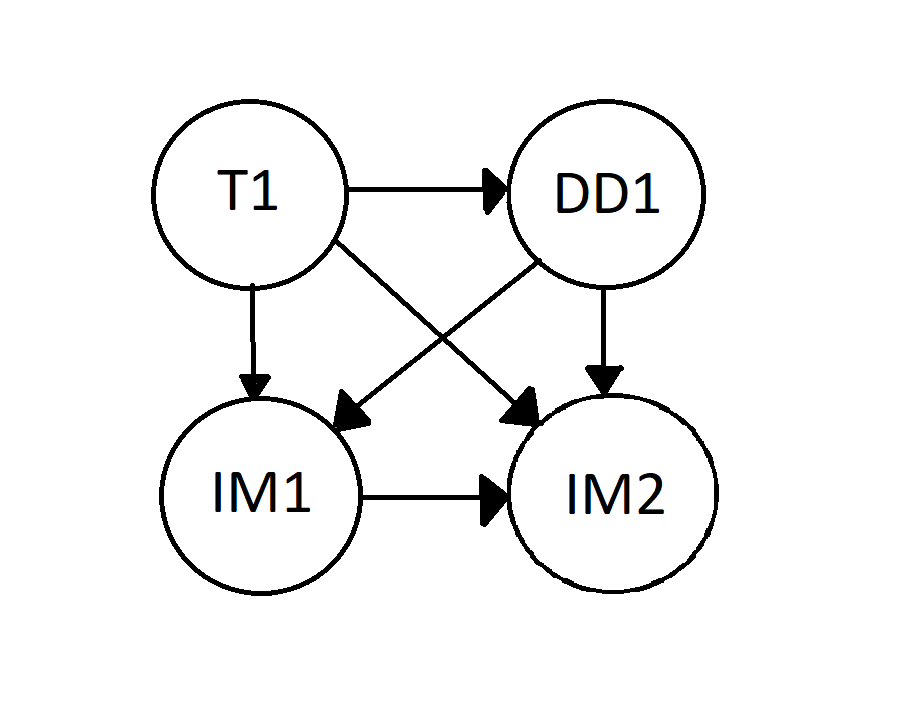
\includegraphics[width=\textwidth]{ATrace.png}
		}
		\caption{\label{Fig_ATrace} Traceability Graph Showing the Connections 
		Between Items of Different Sections}
 	\end{center}
 \end{figure}

\begin{figure}[h!]
	\begin{center}
		{
			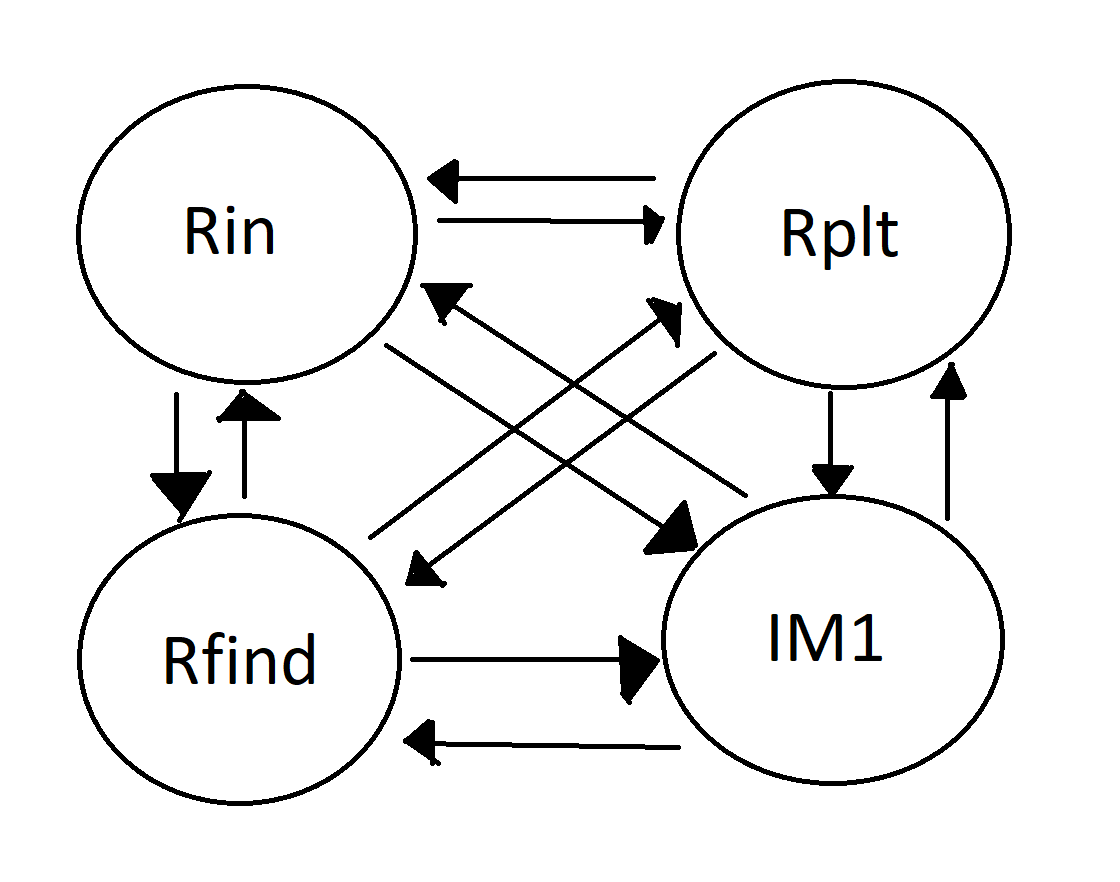
\includegraphics[width=\textwidth]{RTrace.png}
		}
 		\caption{\label{Fig_RTrace} Traceability Graph Showing the Connections 
 			Between Items of Different Sections}
	\end{center}
\end{figure}



%\bibliographystyle {plainnat}
%\bibliography {../../ReferenceMaterial/References} 

\clearpage 
\begin{thebibliography}{9} 
	\bibitem{latexcompanion} 
	Spencer Smith and Lei Lai. 
	A New Requirements Template for Scientific Computing. 
	Proceedings of SREP'05, Paris, France 2005. 
	
	\bibitem{latexcompanion} 
	Spencer Smith, Lei Lai and Ridha Khedri. 
	Requirements Analysis for Engineering computation: A Systematic Approach 
	for Improving Reliability. 
	Springer, 2007. 
	
	\bibitem{latexcompanion} 
	Dmitry E. Pelinovsky. 
	Localization in Periodic Potentials. 
	Cambridge University Press, 2011. 
	
	\bibitem{latexcompanion} 
	Bernard Deconinck and Benjamin L.Segal. 
	The stability spectrum for elliptic solutions to the focusing NLS equation. 
	PhysicaD, 2017.  
	
	\bibitem{latexcompanion} 
	J. Chen and D.E. Pelinovksy. 
	Rogue periodic waves in the focusing nonlinear Schrodinger equation. 
	Proceeding A of Roy.Soc. Lond., 2018. 
	
\end{thebibliography} 

\newpage

\section{Appendix}

\subsection{Symbolic Parameters}

There are no symbolic parameters.

\end{document}